\documentclass[12pt,a4paper]{article}
\usepackage[latin1]{inputenc}
\usepackage[spanish]{babel}
\usepackage{amsmath}
\usepackage{amsfonts}
\usepackage{amssymb}
\usepackage{makeidx}
\usepackage{graphicx}
\usepackage[hidelinks]{hyperref}
\usepackage[left=2cm,right=2cm,top=2cm,bottom=2cm]{geometry}
\author{MEJORADA LOPEZ IVAN}
\title{Dise\~no de un modulacion de ancho pulso(PWM) con Amp-Op y transistores}
\begin{document}
\maketitle

\includegraphics[width=15cm]{UPZMG_Prueba_1b.png} 
\newpage
\section{Que es un PWM}
La modulaci\'in por ancho de pulsos (tambi\'on conocida como PWM, siglas en ingl\'es de pulse-width modulation) de una se\~nal o fuente de energ\'ia es una t\'ecnica en la que se modifica el ciclo de trabajo de una se\~nal peri\'odica (una senoidal o una cuadrada, por ejemplo), ya sea para transmitir informaci\'on a trav\'es de un canal de comunicaciones o para controlar la cantidad de energ\'ia que se env\'ia a una carga.

El ciclo de trabajo de una se\~nal peri\'odica es el ancho relativo de su parte positiva en relaci\'on con el per\'iodo.\\ La construcci\'on t\'ipica de un circuito PWM se lleva a cabo mediante un comparador con dos entradas y una salida. Una de las entradas se conecta a un oscilador de onda dientes de sierra, mientras que la otra queda disponible para la se\~al moduladora. En la salida la frecuencia es generalmente igual a la de la se\~al dientes de sierra y el ciclo de trabajo est\'a en funci\'on de la portadora.

La principal desventaja que presentan los circuitos PWM es la posibilidad de que haya interferencias generadas por radiofrecuencia. Estas pueden minimizarse ubicando el controlador cerca de la carga y realizando un filtrado de la fuente de alimentaci\'on.\\}
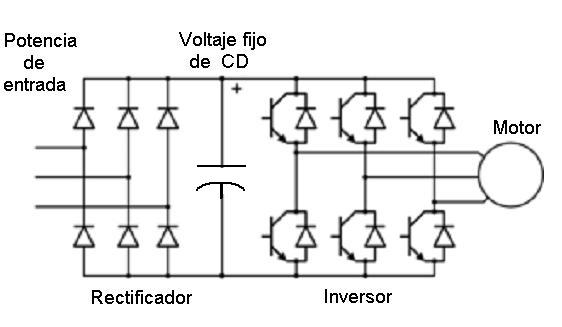
\includegraphics[width=15cm]{Diagrama_variador_de_frecuencia.jpeg} 


\newpage
\section{Para que sirvce un PWM}
Para emular una se\~nal anal\'ogica se cambia el ciclo de trabajo (duty cicle en ingl\'es) de tal manera que el valor promedio de la se\~nal sea el voltaje aproximado que se desea obtener, pudiendo entonces enviar voltajes entre 0[V] y el m\'aximo que soporte el dispositivo PWM utilizado, en el caso de Arduino es 5[V].\\
Las aplicaciones t\'ipicas para este tipo de se\~nales son: Controlar intensidad de un LED, mover servomotores, controlar LED RGB, controlar velocidad de motores de corriente continua y controlar motores el\'ectricos de inducci\'on o asincr\'onicos.\\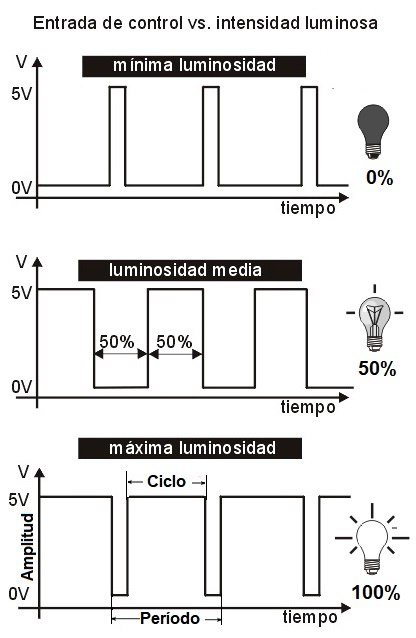
\includegraphics[width=10cm]{Tabla_Pwm.jpg}  
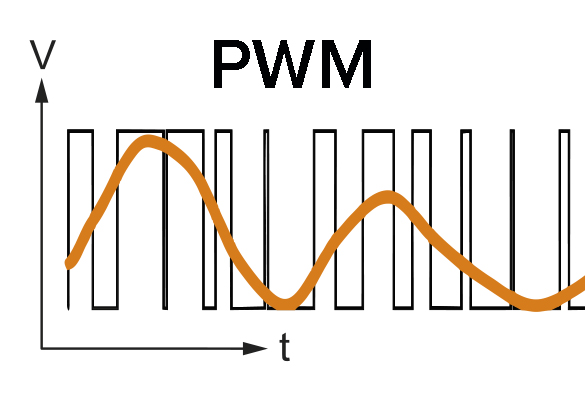
\includegraphics[width=10cm]{What-is-PWM-585x400.jpg}\\
\newpage
En este apartado veremos un peque\~no resumen de lo que es un PWM con un Amp-Omp como se muestra en la siguiente imagen, podemos observar su onda que se marca en un ociloscopio y el diagrama puesto en marcha\\ 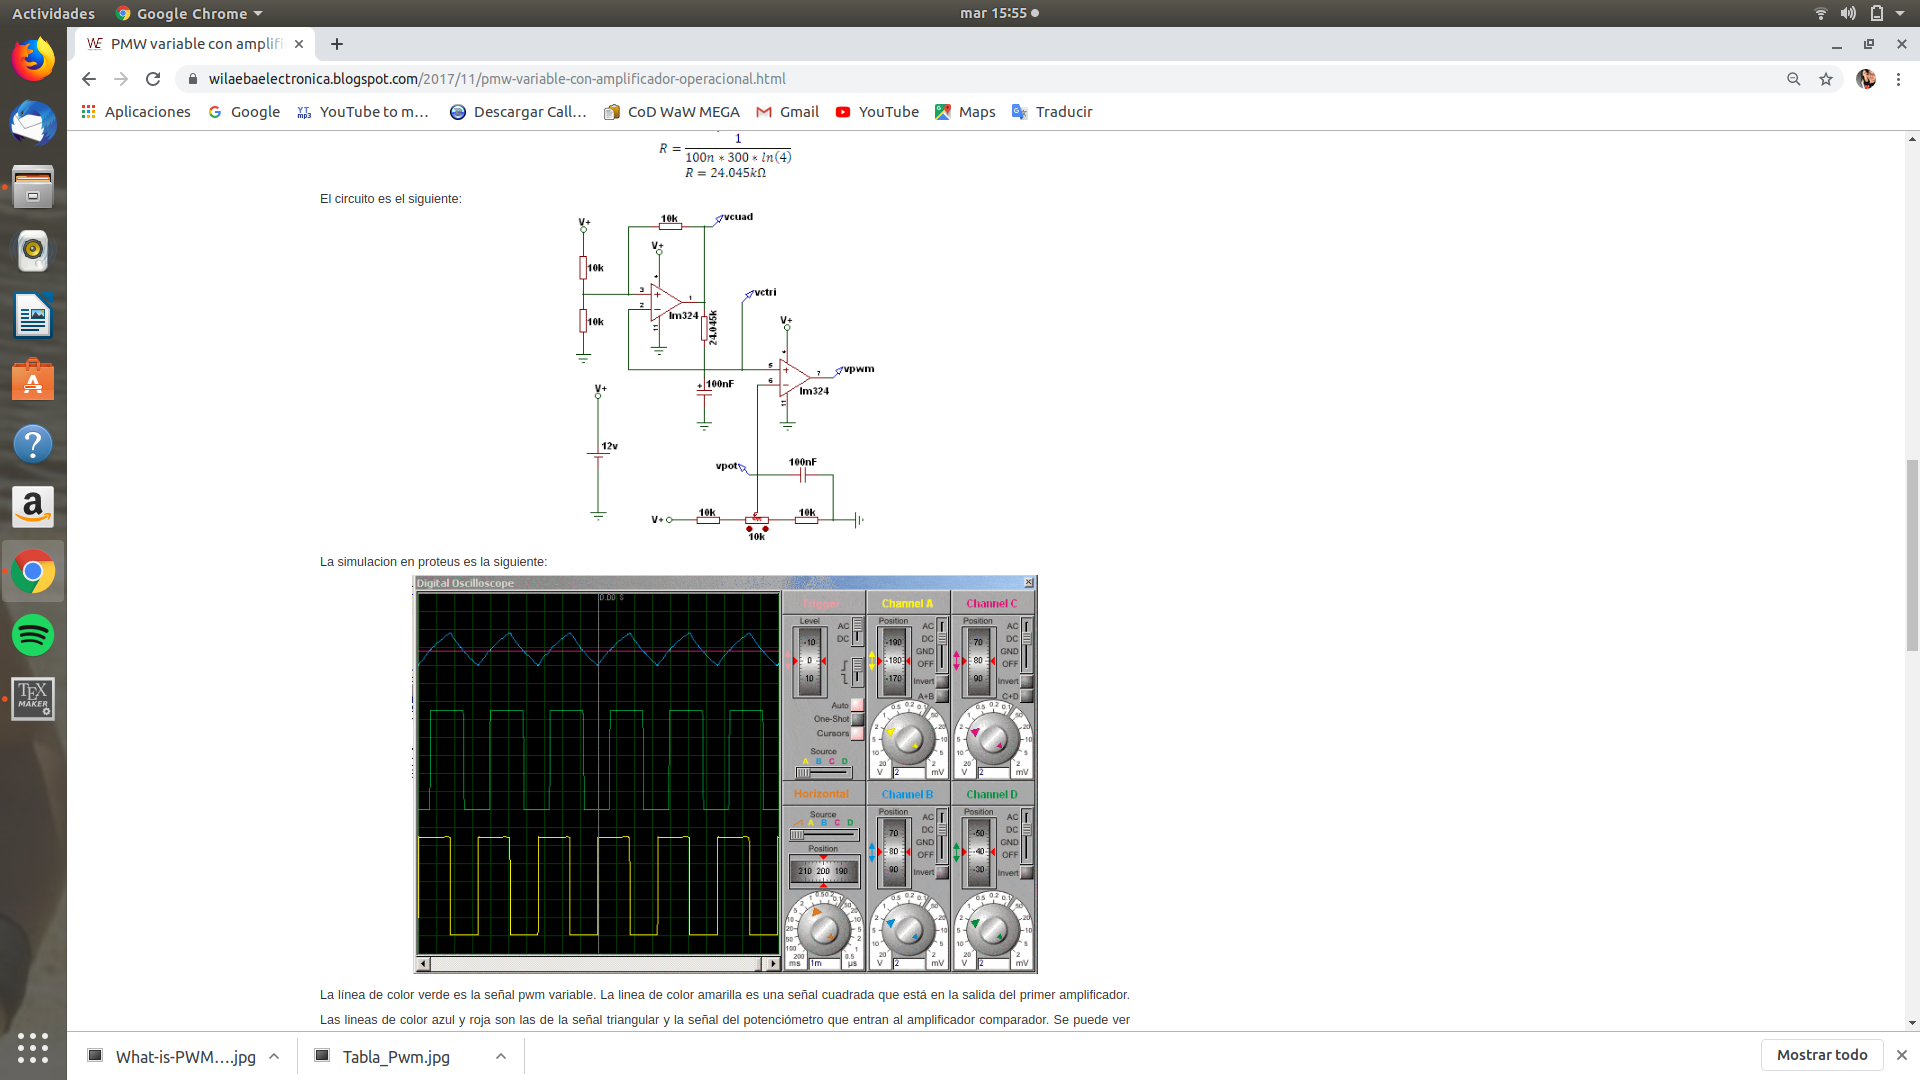
\includegraphics[width=15cm]{Captura-de-pantalla-de-2019-10-22-15-55-18.png} 
\\
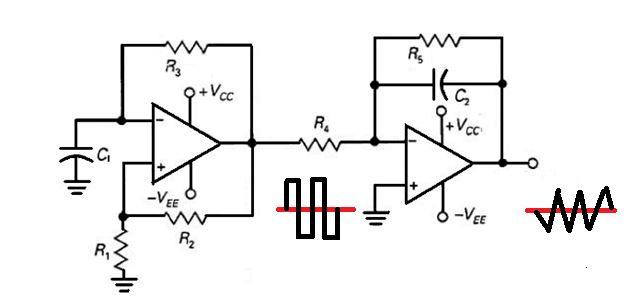
\includegraphics[width=15cm]{captura.jpg} 

\section{bibliografias}

\url{http://www.arduino.utfsm.cl/modulacion-por-ancho-de-pulso-pwm/}\\
\url{https://es.wikipedia.org/wiki/Modulaci}\%C3\%B3n_por_ancho_de_pulsos}



 

\end{document}